% !TeX root = ../main.tex

\chapter{实验与分析}
本章将依据建立好的样本库,对第三章相关问题进行实验验证,并根据计算出的云图特征,
提出能够提取雷暴云的图像特征阈值范围。

\section{传感器不同波段的实验验证}
由于不同通道波段不同,在图像上所表示的纹理特征也各有差异,
下面将对不同通道不同波段的特征进行分析比较。选取分辨率为25像素,雷暴云强度选取10$\sim$15之间,纹理特征取eng和idm。
14个波段的散点图如图5.1所示。

\begin{figure}
    \centering
    \subfigure{
    \begin{minipage}[t]{0.45\linewidth}
    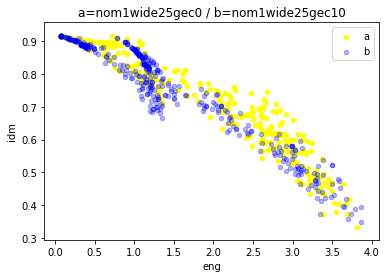
\includegraphics[width=1\linewidth,height=0.5\linewidth]{431.png}\vspace{2pt}
    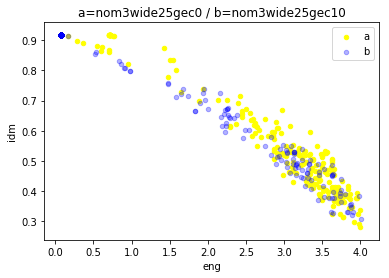
\includegraphics[width=1\linewidth,height=0.5\linewidth]{433.png}\vspace{2pt}
    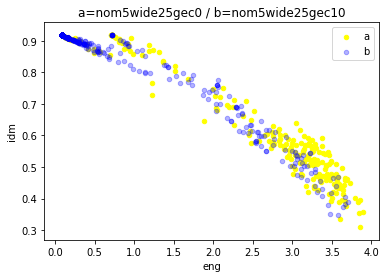
\includegraphics[width=1\linewidth,height=0.5\linewidth]{435.png}\vspace{2pt}
    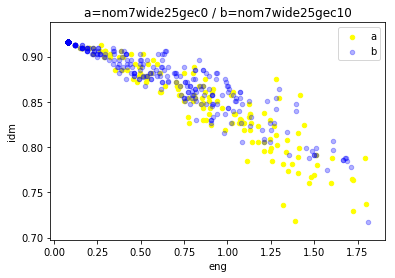
\includegraphics[width=1\linewidth,height=0.5\linewidth]{437.png}\vspace{2pt}
    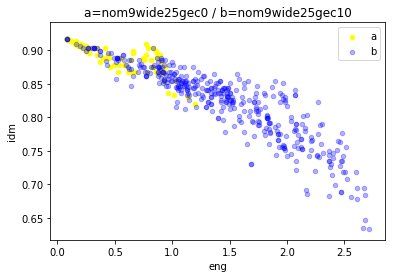
\includegraphics[width=1\linewidth,height=0.5\linewidth]{439.png}\vspace{2pt}
    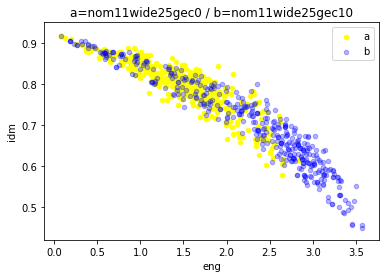
\includegraphics[width=1\linewidth,height=0.5\linewidth]{4311.png}\vspace{2pt}
    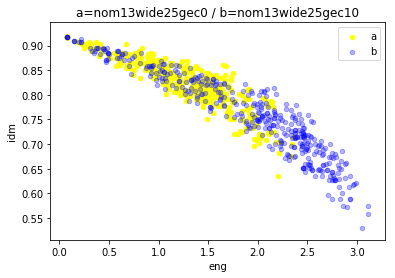
\includegraphics[width=1\linewidth,height=0.5\linewidth]{4313.png}
    \end{minipage}}
    \subfigure{
    \begin{minipage}[t]{0.45\linewidth}
    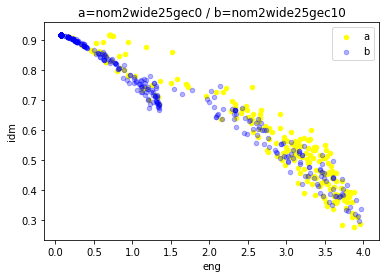
\includegraphics[width=1\linewidth,height=0.5\linewidth]{432.png}\vspace{2pt}
    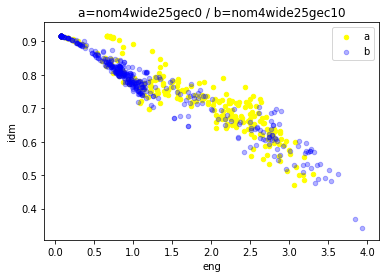
\includegraphics[width=1\linewidth,height=0.5\linewidth]{434.png}\vspace{2pt}
    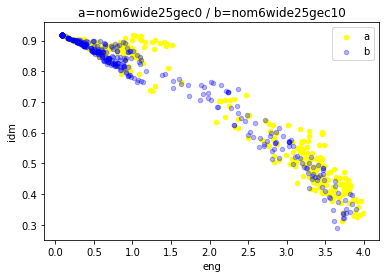
\includegraphics[width=1\linewidth,height=0.5\linewidth]{436.png}\vspace{2pt}
    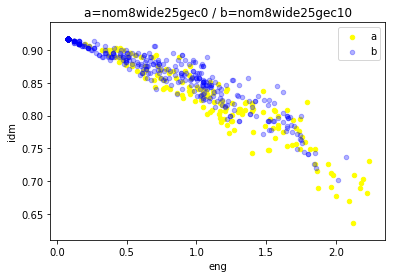
\includegraphics[width=1\linewidth,height=0.5\linewidth]{438.png}\vspace{2pt}
    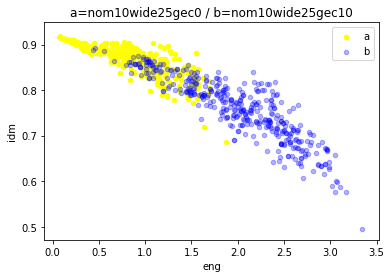
\includegraphics[width=1\linewidth,height=0.5\linewidth]{4310.png}\vspace{2pt}
    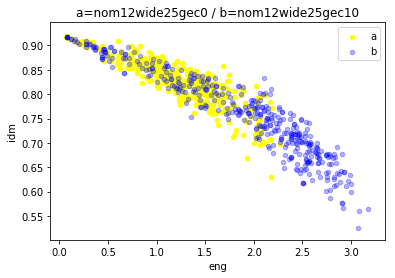
\includegraphics[width=1\linewidth,height=0.5\linewidth]{4312.png}\vspace{2pt}
    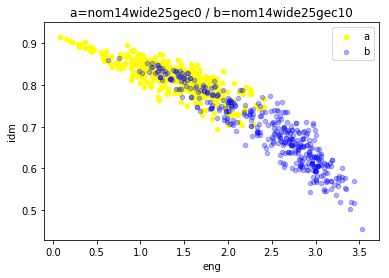
\includegraphics[width=1\linewidth,height=0.5\linewidth]{4314.png}
    \end{minipage}}
    \caption{不同波段纹理特征比较}
  \end{figure}

分析散点图可得:

1.低通道部分雷暴云类似线性聚集在一起,分析图像后发现,可见光通道和近红外通道在夜晚无法成像,
因此计算得出的纹理特征较为聚集。

2.观察5$\sim$10通道发现,雷暴云特征渐渐向图像右下方聚集,分析后得出,9、10通道介于中波红外与长波红外之间,
可以反映雷暴天气中的中高层水汽。

3.观察散点图可以发现中波红外到长波红外相比可见光和近红外更能反映雷暴信息。

实验证明了第三章提出的,在中长波红外和水汽通道能够较好反映出雷暴信息的结论。

\section{雷暴尺度及强度问题的实验验证}
\subsection{雷暴尺度问题}
图5.2中,nom1即表示1通道,共14个通道,wide25和wide50分别表示图像分辨率为25像素和50像素,
gec5表示雷暴强度大于5,将相同通道,相同雷暴强暴,相同纹理特征量(asm和con),
不同分辨率图像的纹理数据以散点图的形式表示,通过比较不同分辨率的图像,可以发现50像素分辨率相比25像素分辨率图像,
在各个通道都更为聚集。

\begin{figure}
    \centering
    \subfigure{
    \begin{minipage}[t]{0.45\linewidth}
    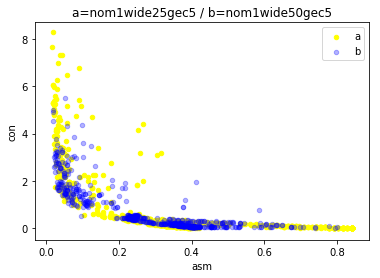
\includegraphics[width=1\linewidth,height=0.5\linewidth]{411.png}\vspace{2pt}
    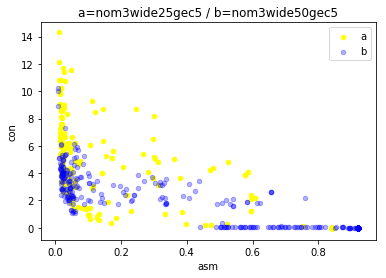
\includegraphics[width=1\linewidth,height=0.5\linewidth]{413.png}\vspace{2pt}
    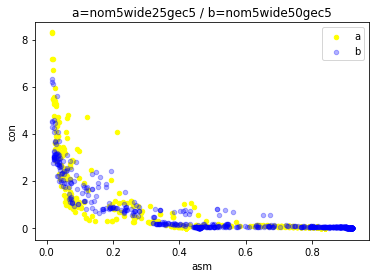
\includegraphics[width=1\linewidth,height=0.5\linewidth]{415.png}\vspace{2pt}
    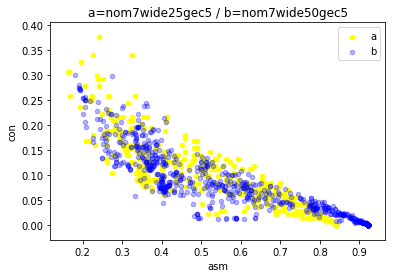
\includegraphics[width=1\linewidth,height=0.5\linewidth]{417.png}\vspace{2pt}
    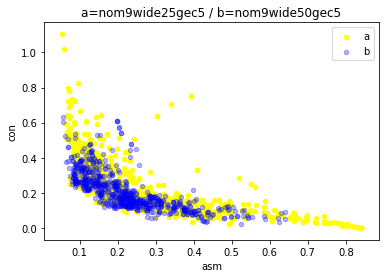
\includegraphics[width=1\linewidth,height=0.5\linewidth]{419.png}\vspace{2pt}
    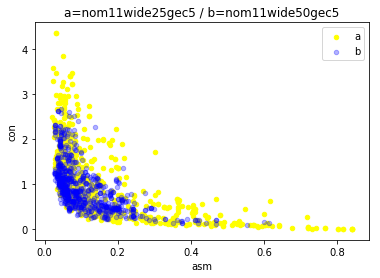
\includegraphics[width=1\linewidth,height=0.5\linewidth]{4111.png}\vspace{2pt}
    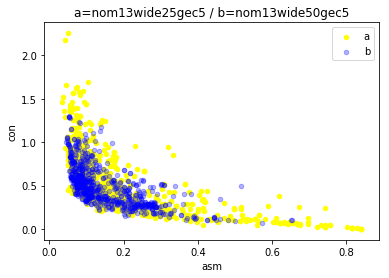
\includegraphics[width=1\linewidth,height=0.5\linewidth]{4113.png}
    \end{minipage}}
    \subfigure{
    \begin{minipage}[t]{0.45\linewidth}
    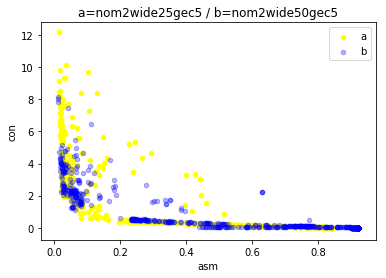
\includegraphics[width=1\linewidth,height=0.5\linewidth]{412.png}\vspace{2pt}
    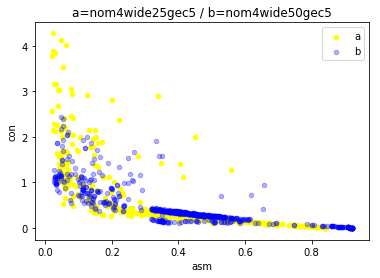
\includegraphics[width=1\linewidth,height=0.5\linewidth]{414.png}\vspace{2pt}
    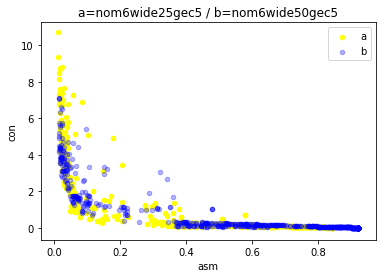
\includegraphics[width=1\linewidth,height=0.5\linewidth]{416.png}\vspace{2pt}
    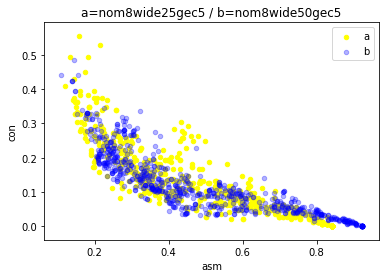
\includegraphics[width=1\linewidth,height=0.5\linewidth]{418.png}\vspace{2pt}
    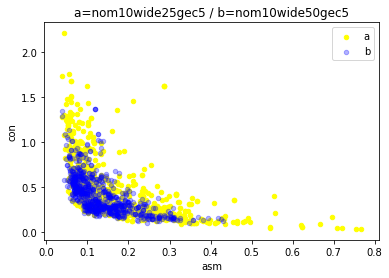
\includegraphics[width=1\linewidth,height=0.5\linewidth]{4110.png}\vspace{2pt}
    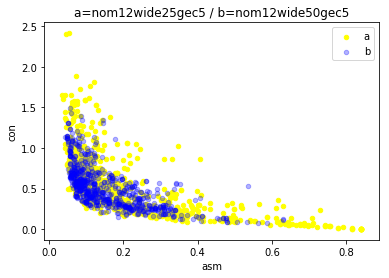
\includegraphics[width=1\linewidth,height=0.5\linewidth]{4112.png}\vspace{2pt}
    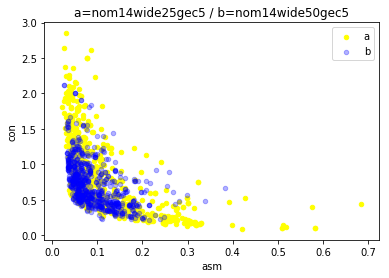
\includegraphics[width=1\linewidth,height=0.5\linewidth]{4114.png}
    \end{minipage}}
    \caption{不同分辨率纹理特征比较}
  \end{figure}

\subsection{雷暴强度问题}
雷暴强度为闪电仪中获取到的闪电辐射值,下面将分析不同雷暴强度的图像,gec5表示雷暴强度介于5$\sim$10之间(标准化后数值),
gec10表示雷暴强度介于10$\sim$15之间,选取分辨率为25像素,纹理特征量取con和idm,各通道散点图如图5.3所示。

由各通道散点图可以看出,雷暴强度大于10的纹理特征相比雷暴强度介于5$\sim$10之间的纹理特征更为明显。


\begin{figure}
    \centering
    \subfigure{
    \begin{minipage}[t]{0.45\linewidth}
    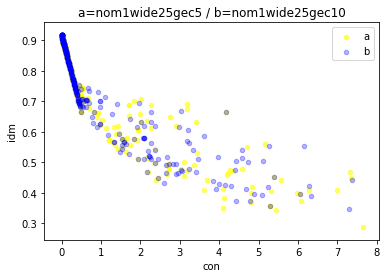
\includegraphics[width=1\linewidth,height=0.5\linewidth]{421.png}\vspace{2pt}
    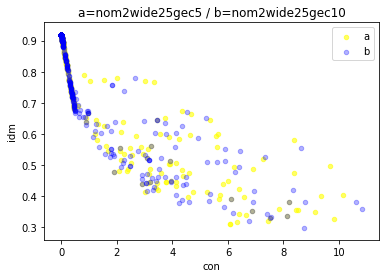
\includegraphics[width=1\linewidth,height=0.5\linewidth]{423.png}\vspace{2pt}
    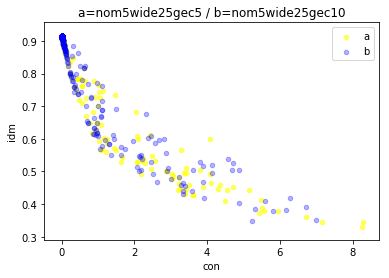
\includegraphics[width=1\linewidth,height=0.5\linewidth]{425.png}\vspace{2pt}
    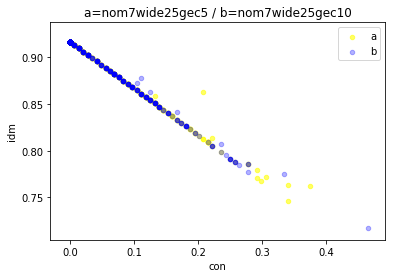
\includegraphics[width=1\linewidth,height=0.5\linewidth]{427.png}\vspace{2pt}
    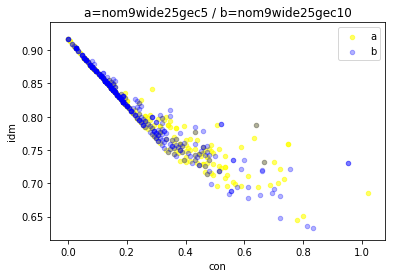
\includegraphics[width=1\linewidth,height=0.5\linewidth]{429.png}\vspace{2pt}
    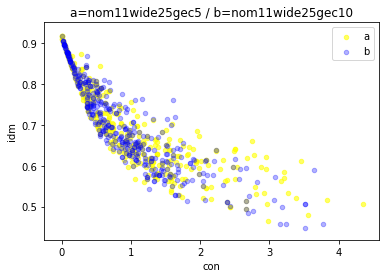
\includegraphics[width=1\linewidth,height=0.5\linewidth]{4211.png}\vspace{2pt}
    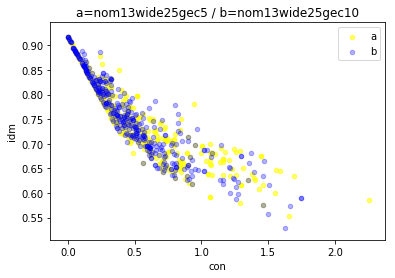
\includegraphics[width=1\linewidth,height=0.5\linewidth]{4213.png}
    \end{minipage}}
    \subfigure{
    \begin{minipage}[t]{0.45\linewidth}
    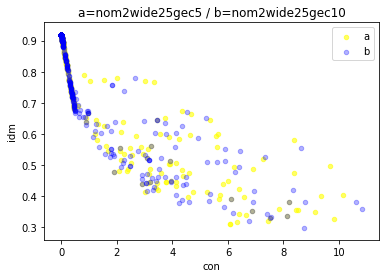
\includegraphics[width=1\linewidth,height=0.5\linewidth]{422.png}\vspace{2pt}
    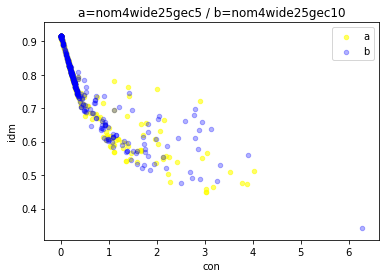
\includegraphics[width=1\linewidth,height=0.5\linewidth]{424.png}\vspace{2pt}
    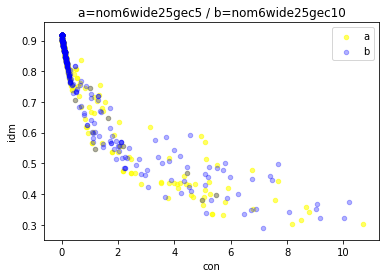
\includegraphics[width=1\linewidth,height=0.5\linewidth]{426.png}\vspace{2pt}
    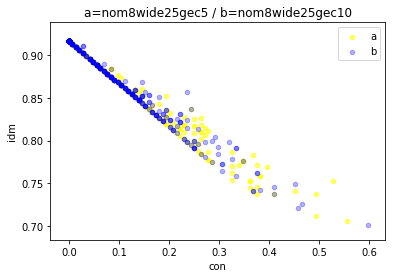
\includegraphics[width=1\linewidth,height=0.5\linewidth]{428.png}\vspace{2pt}
    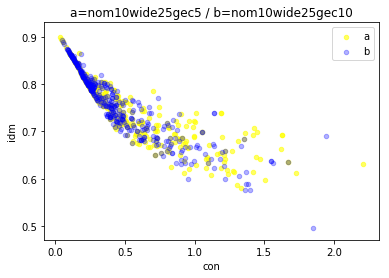
\includegraphics[width=1\linewidth,height=0.5\linewidth]{4210.png}\vspace{2pt}
    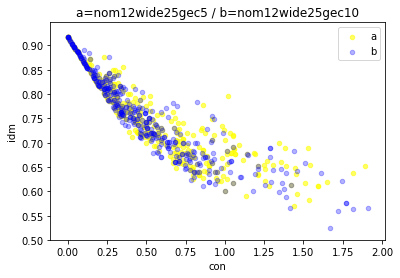
\includegraphics[width=1\linewidth,height=0.5\linewidth]{4212.png}\vspace{2pt}
    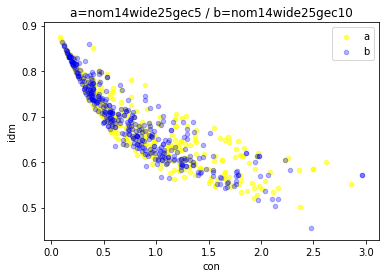
\includegraphics[width=1\linewidth,height=0.5\linewidth]{4214.png}
    \end{minipage}}
    \caption{不同雷暴强度纹理特征比较}
  \end{figure}

\section{纹理特征融合实验分析}
本文共计算了灰度共生矩阵的四种统计量,分别为asm,con,eng,idm,其中两两组合可以输出联合散点图,
共六种组合方式,选取第10通道,分辨率25,将非雷暴云和雷暴云进行比较,各通道散点图如图5.4所示。

由散点图可得,idm与eng联合,con与asm联合,asm与eng联合能够较为准确的反映雷暴云特征。

\begin{figure}
    \centering
    \subfigure{
    \begin{minipage}[t]{0.45\linewidth}
    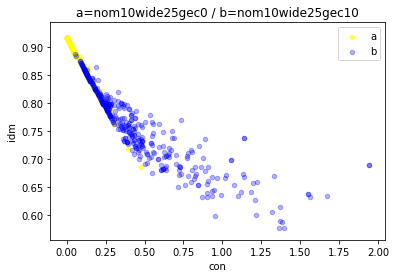
\includegraphics[width=1\linewidth,height=0.5\linewidth]{441.png}\vspace{2pt}
    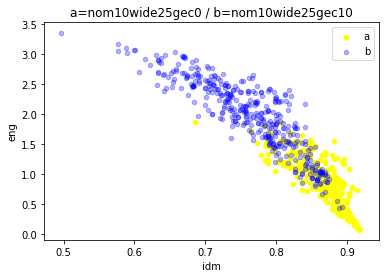
\includegraphics[width=1\linewidth,height=0.5\linewidth]{443.png}\vspace{2pt}
    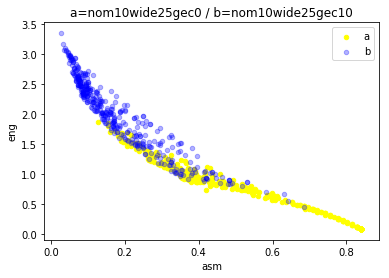
\includegraphics[width=1\linewidth,height=0.5\linewidth]{445.png}
    \end{minipage}}
    \subfigure{
    \begin{minipage}[t]{0.45\linewidth}
    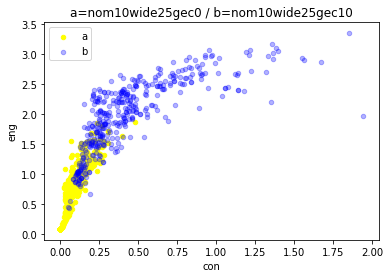
\includegraphics[width=1\linewidth,height=0.5\linewidth]{442.png}\vspace{2pt}
    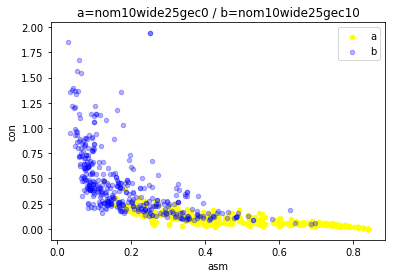
\includegraphics[width=1\linewidth,height=0.5\linewidth]{444.png}\vspace{2pt}
    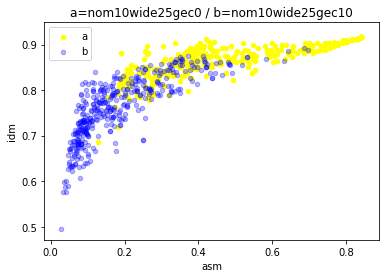
\includegraphics[width=1\linewidth,height=0.5\linewidth]{446.png}
    \end{minipage}}
    \caption{不同波段纹理特征比较}
  \end{figure}


\section{阈值提取}
针对以上分析,挑选出雷暴云与非雷暴云分类较为明显的散点图,如图5.5。

\begin{figure}
    \centering
    \subfigure{
    \begin{minipage}[t]{0.45\linewidth}
    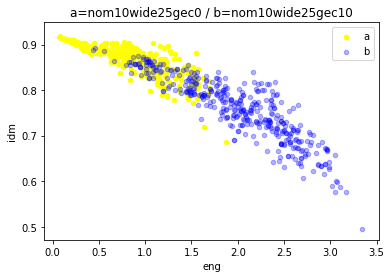
\includegraphics[width=1\linewidth,height=0.5\linewidth]{451.png}\vspace{2pt}
    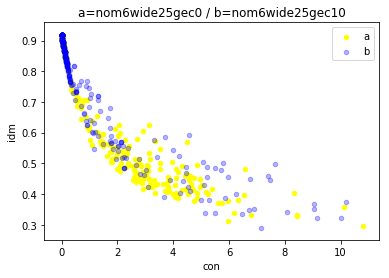
\includegraphics[width=1\linewidth,height=0.5\linewidth]{453.png}\vspace{2pt}
    \includegraphics[width=1\linewidth,height=0.5\linewidth]{455.png}
    \end{minipage}}
    \subfigure{
    \begin{minipage}[t]{0.45\linewidth}
    \includegraphics[width=1\linewidth,height=0.5\linewidth]{452.png}\vspace{2pt}
    \includegraphics[width=1\linewidth,height=0.5\linewidth]{454.png}\vspace{2pt}
    \includegraphics[width=1\linewidth,height=0.5\linewidth]{456.png}
    \end{minipage}}
    \caption{分类效果较好的散点图}
  \end{figure}

根据效果较好的散点图,提出了如下纹理特征阈值范围。
\begin{equation}
    0.78<eng(nom10)<3.50
\end{equation}
\begin{equation}
    0.09<con(nom10)<2.00 
\end{equation}
\begin{equation}
    0.50<idm(nom10)<0.90
\end{equation}
\begin{equation}
    0<asm(nom10)<0.40
\end{equation}

联合以上阈值范围,在一个包含400张雷暴云和400张非雷暴云的测试库中进行检测,
可以检测出370张雷暴图,119张非雷暴图,预警率为92.5$\%$,虚警率为29.75$\%$,
漏判率为24.34$\%$。